% Compiled with TeXLive 2011.
\synctex=1
\documentclass[a4paper,11pt]{amsart}

\usepackage[a4paper]{geometry}
\usepackage[backend=biber,citestyle=authoryear]{biblatex}
\usepackage{amsmath}
\usepackage{amssymb}
\usepackage{float}
\usepackage{setspace}
\usepackage{mathrsfs}
\usepackage{color}
\usepackage{graphicx}
\usepackage{psfrag}
\usepackage{siunitx}
\usepackage{caption}
\usepackage{multirow}
\usepackage{hyperref}
\usepackage{subfigure}
\usepackage{algorithms/algorithm}
\usepackage{algorithms/algorithmic}
\usepackage[english]{babel}
\usepackage[nice]{nicefrac}
\usepackage{fancybox}
\usepackage{multicol}
\usepackage{pgf}
\usepackage{tikz}
\usepackage{tikz-qtree}
\usepackage{lscape}
\usepackage{rotating}
\usepackage{enumerate}
\usepackage{pgfplots,tikz}
\usepackage{listings}

\usepackage[utf8]{inputenc}
\usepackage[T1]{fontenc}
\usepackage[sc]{mathpazo}


\newenvironment{frcseries}{\fontfamily{frc}\selectfont}{}
\newcommand{\textfrc}[1]{{\frcseries#1}}
\newcommand{\mathfrc}[1]{\textit{\textfrc{#1}}}

\usepackage{rotating}

\makeatletter
\newenvironment{sqcases}{%
  \matrix@check\sqcases\env@sqcases
}{%
  \endarray\right.%
}
\def\env@sqcases{%
  \let\@ifnextchar\new@ifnextchar
  \left\lbrack
  \def\arraystretch{1.2}%
  \array{@{}l@{\quad}l@{}}%
}
\makeatother

\newcommand\xput[2][0.5]{%
    \rule{#1\linewidth}{0pt}\makebox[0pt][c]{#2}\hfill}


\sisetup{table-format=3.2, % Adjust for needed decimal places
    table-number-alignment=center % Centers the numbers
}

\captionsetup{skip=10pt}

\setlength{\parindent}{0pt}

\makeatletter
\newcommand{\addresseshere}{%
  \enddoc@text\let\enddoc@text\relax
}
\makeatother

\newlength\figureheight
\newlength\figurewidth

\newcommand{\Dynare}{\href{http://www.dynare.org}{Dynare}}

\addbibresource{dsge.bib}

\pdfcompresslevel=9

\hypersetup{bookmarks=false,
    unicode=true,
    pdftoolbar=false,
    pdfmenubar=false,
    pdffitwindow=true,
    pdfstartview={FitH},
    pdftitle={Stochastic Extended Path},
    pdfauthor={Stéphane Adjemian},
    pdfcreator={Stéphane Adjemian},
    pdfproducer={pdflatex},
    colorlinks=true,
    linkcolor=blue,
    citecolor=blue,
    filecolor=blue,
    urlcolor=blue
}

% ----------------------------------------------------------------



% ---------------------------------------------------------------- %\maketitle % ----------------------------------------------------------------
\begin{document}

\author[S. Adjemian]{Stéphane Adjemian}\address{Université du Mans and Dynare team}\email{stephane.adjemian@univ-lemans.fr}
\author[M. Juillard]{Michel Juillard}\address{Dynare team}\email{michel.juillard@mjui.fr}


\title[Stochastic Extended Path]{Stochastic Extended Path}\thanks{}
\date{December, 2016}
\maketitle

\section*{Introduction}

The extended path approach, initially introduced by
\textcite{FairTaylor1983} and implemented in \Dynare, utilizes perfect
foresight model solvers to effectively address deterministic
nonlinearities related to preferences, technology functional forms, or
occasionally binding constraints. In each period of the simulation,
exogenous innovations are treated as surprise shocks occurring in the
first period of a deterministic simulation, with shocks thereafter set
to their expected values. This approach offers significant advantages
over other global approximation methods, including the ability to
simulate very large models and its simplicity, as it is not
model-dependent and requires no more effort than composing a \Dynare\,
\verb+*.mod+ file.\newline

This approach, which relies on perfect foresight model solvers,
inherently overlooks Jensen's inequality. While the extended path
method can handle deterministic non-linearity with arbitrary
precision, it remains unaddressed regarding stochastic
non-linearity. Since future shocks are anticipated to equal their
expectations, current agent behavior is unaffected by future
uncertainty. According to \textcite{Gagnon1990} and
\textcite{Love2009}, who analyze an RBC model, this approximation has
minimal effects. However, \textcite{AdjemianJuillard2011}
demonstrated, in the context of an NK model with a zero lower bound on
nominal interest rates, that neglecting future uncertainty is
inconsequential only when the interest rate constraint is
non-binding. In this paper, we propose relaxing the assumption about
future shocks by employing numerical integration to approximate
conditional expectations.\newline

The Stochastic Extended Path approach (SEP), similar to the
deterministic Extended Path approach, generates time series for the
model's endogenous variables without explicitly calculating a reduced
form that links choice variables to state variables\footnote{Note
   however that, in a subsequent stage, one can estimate this
   relationship using the time series generated by the SEP
   approach. The fitted polynomial can serve as an initial guess for
   the Parameterized Expectations Algorithm or be used to extend the
   simulation with significantly reduced computational costs.}. This
method is advantageous in cases where the model's reduced form is
poorly behaved due to high non-linearity or kinks, which makes it
challenging to approximate. However, a drawback is that it does not
leverage the problem's recursive structure, limiting its ability to
fully account for future uncertainty. Specifically, it requires
integration over shocks in all future periods, which may not be feasible.\footnote{Note that the pertubation
   approach fully account for future uncertainty conditionally on a
   given approximation order, in this sense it does not account for all
   the future uncertainty.}.
The Stochastic Extended Path of order \( p \) simplifies future
uncertainty by positing that shocks will occur in the next \( p \)
periods, with subsequent shocks set to their expected
values.  Agents then expect that the
economy goes back to the deterministic steady state.\newline

Section~\ref{sec:1} introduces the class of models being examined and
the Extended Path approach. Section~\ref{sec:2} addresses
modifications to the Extended Path approach to incorporate the impact
of future uncertainty. Additionally, we conduct accuracy checks using
a model where future uncertainty is significant and for which a
closed-form solution is available. Section~\ref{sec:3} presents a
numerical illustration considering a Real Business Cycle (RBC) model
with irreversible investment.

\section{Extended Path}\label{sec:1}

We assume that the model can be expressed in the following manner:
\begin{equation}\label{eq:model}
   \mathbb E_t\left[f\left( y_{t-1}, y_t, y_{t+1}, \varepsilon_t \right)\right] = 0
\end{equation}

where \( y_t \) is an \( n \times 1 \) vector of endogenous
variables, \( \varepsilon_t \) is an \( n_s \times 1 \) vector of
innovations, and \( f: \mathbb R^{3n+n_s} \rightarrow \mathbb R^n \)
is a continuous function. The innovations are assumed to be
independent and identically distributed and follow a Gaussian
distribution: \( \mathcal N(0,\Sigma) \). The assumption regarding the
distribution of innovations can be relaxed; however, this would
necessitate the use of different quadrature rules in section~\ref{sec:2}. The conditional expectation is presented above the
function $f$, but we could readily extend this to consider conditional
expectations under a nonlinear function by incorporating additional
auxiliary variables. Similarly, we could address an arbitrary number
of lags or leads by utilizing auxiliary variables. We do not assume
that the function \(f\) is differentiable everywhere, which is why the
extended path approach can accommodate scenarios where the left and
right derivatives differ due to occasionally binding
constraints. Nevertheless, it is evident that solving a model is
always easier when \(f\) is differentiable at all points. We also
assume that the model has a deterministic steady state and that the
economy converges to this steady state in the long run. There exists a
vector of endogenous variables \(y^{\star}\) such that:
\[
   f\left(y^{\star},y^{\star},y^{\star}, 0\right) = 0
\]
and $\lim_{h\rightarrow\infty}y_{t+h} = y^{\star}$ for all $y_{t-1}$.
This assumption could be relaxed; what is essential is a terminal
condition for the endogenous variables. As long as we know where the
economy goes in the long run (for instance, along a balanced growth
path), the method described below can be accommodated.

\subsection{Perfect foresight model}\label{sec:pf}

Perfect foresight models are commonly employed to generate impulse
response functions. Starting with an initial condition \(y_{t-1}\) and
an unexpected shock occurring in period \(t\), \(\varepsilon_t\), we
aim to find the trajectory of the endogenous variables under the
assumptions that \emph{(i)} subsequent shocks are set to their
expected values, \emph{(ii)} the model reaches the steady
state \(y^*\) in period \(t+H\).

\begin{equation}\label{eq:pf}
   \begin{cases}
      f\left(y_{t-1},y_t,y_{t+1},\varepsilon_t\right) = 0                            \\
      f\left(y_{t-1+h}, y_{t+h}, y_{t+h+1}, 0\right) =0 \quad\forall\, h=0,\dots,H-2 \\
      f\left(y_{t+H-2}, y_{t+H-1}, y^{\star}, 0\right) =0
   \end{cases}
\end{equation}

\smallskip\smallskip

Comparing this system of equations to equation \eqref{eq:model},
assumption \emph{(i)} suggests that it is legitimate to pass the
expectation operator inside the function \(f\). This is obviously a
crude approximation, since \(f\) is a priori a non-linear
funtion. Assumption \emph{(ii)} is less concerning, as the distance to
the steady state can be made arbitrarily small with a sufficiently
large simulation horizon, $H$.\newline

Concatenating all the vectors of endogenous variables in
the \(nH\times 1\)
vector \(Y_t = \left(y_t',y_{t+1}', \ldots, y_{t+H-1}' \right)\)' the
system of equations to be solved can be written as:
\[
   F(Y_t) = 0
\]
where $F: \mathbb{R}^{nH} \rightarrow \mathbb{R}^{nH}$ is a function
that aggregates the functions $f$ across all
periods. \textcite{Laffargue1990} demonstrates that perfect foresight
models can be solved using Newton-type methods, taking advantage of
the sparse structure of the Jacobian of $F$, which is block
tridiagonal. In the Newton approach, the solution for vector Y is
found iteratively. For an initial guess $Y_t^{(0)}$, usually the
steady state or a path generated by a first order apporoximation of
the model, successive approximated solutions $Y_t^{(k)}$ are obtained
by solving the following linear problem:
\[
   F\left( Y_t^{(k)} \right) + J_F\left(Y_t^{(k)}\right) \left( Y_t^{(k+1)} - Y_t^{(k)} \right)  = 0
\]
where $J_F\left(Y_t^{(k)}\right)$ is the Jacobian matrix of $F$
evaluated at the current trajectory for the endogenous
variables $Y_t^{(k)}$. With current computers, standard algorithms for
solving sparse linear problems, such as those developed by
\textcite{Davis2006}, and available in Matlab or Octave, for example,
can be used very efficiently in this framework.\newline

\subsection{Extended path algorithm}

To simulate stochastic models, \textcite{FairTaylor1983} propose the
following approach: for each period in the stochastic simulation, draw
a random vector of stochastic shocks \(\varepsilon_t\); run an
auxiliary deterministic version of the model\footnote{It is important
   to note that we employ a relaxation method to solve the perfect
   foresight auxiliary model in Dynare, while \textcite{FairTaylor1983}
   utilized a shooting method, which is known to be less efficient and
   accurate.}, assigning the shocks in the first period
to \(\varepsilon_t\) while setting all future shocks to zero; then,
use the values of the endogenous variables from the first period of
this auxiliary model as the values of the endogenous variables in
period \(t\) of the stochastic simulation. Below is a sketch of the algorithm:\newline

\algsetup{linenosize=\small,
   linenodelimiter=.
}
\begin{algorithm}[H]
   \caption{Extended path algorithm}
   \label{alg:ep}
   \begin{algorithmic}[1]
      \STATE $H \leftarrow$ Set the horizon of the perfect foresight models
      \STATE $y_0 \leftarrow$ Choose an initial condition
      \FOR{$t=1$ to $T$}
      \STATE $\varepsilon_t \leftarrow$ Draw a random vector from a gaussian distribution  $\mathcal N\left(0, \Sigma\right)$
      \STATE $y_t \leftarrow$ Solve the auxiliary perfect foresight model using \(y_{t-1}\) as the initial condition, with the terminal condition \(y_{t+H} = y^{\star}\)
      \ENDFOR
   \end{algorithmic}
\end{algorithm}

\smallskip\smallskip

In iteration \(t\) of the main loop, the initial guess for the
auxiliary perfect foresight model solver is constructed from the
solution of the same model in step \(t-1\). In this approach,
conditional expectations are approximated by setting the shocks to
zero, their expected value. This method overlooks Jensen's inequality
and simulates a stochastic scenario based on a form of certainty
equivalence. Whether this poses a problem depends on the specific
model being used. It is important to note that a perturbation approach
utilizing a first-order approximation of the model would encounter
similar limitations, failing to address the deterministic nonlinearity
inherent in the model. In contrast, the Extended Path approach accepts
certainty equivalence as a trade-off for comprehensively accounting
for the deterministic nonlinearity. Another advantage of this approach
is its ability to accurately simulate models with variables that
significantly deviate from the deterministic steady state, where
perturbation methods would yield inaccurate solutions. Finally, in
contrast to perturbation-based solutions, this approach enables the
incorporation of an arbitrary number of occasionally binding
constraints, as we do not require the differentiability
of \(f\).\newline

The Extended Path approach allows for the simulation of large models
with arbitrary precision, as the number of required operations
increases only polynomially with the number of endogenous variables
(the primary task when solving the auxiliary perfect foresight model
consists in solving a sparse system of linear equations). This
contrasts with a global approximation of the policy rules or
expectations, where the complexity grows exponentially. The Extended
Path approach is not affected by the so-called curse of dimensionality
concerning the number of state variables.\newline

\section{Stochastic Extended Path}\label{sec:2}

\subsection{Numerical integration}

To accommodate non-zero shocks in periods $t+1$, $t+2$, \dots, $t+p$
($p \geq 1$), it is necessary to explicitly compute the (conditional)
expectations for the periods $t$, $t+1$, \dots, $t+p-1$. Different
numerical approaches are available to achieve this.\newline


\subsubsection{Gaussian quadrature}
Let $X$ be a Gaussian random
variable with mean zero and variance $\sigma^2_x > 0$. We aim to
evaluate $\mathbb{E}[\varphi(X)]$, where $\varphi$ is a continuous
function. The expectation can be expressed as follows, utilizing the
Gaussian probability density function:

\[
   \mathbb{E}[\varphi(X)] = \frac{1}{\sigma_x \sqrt{2\pi}} \int_{-\infty}^{\infty} \varphi(x) e^{-\frac{x^2}{2\sigma^2_x}} \mathrm{d}x.
\]

This integral can be approximated using a well-established result (see
\cite{JuddBook1998}):

\[
   \int_{-\infty}^{\infty} \phi(x) e^{-x^2} \mathrm{d}x = \sum_{i=1}^m \omega_i \phi(x_i) + \frac{m! \sqrt{m}}{2^m} \frac{\phi^{(2m)}(\xi)}{(2m)!}
\]

for any $\xi \in \mathbb{R}$. Here, the last term on the right-hand
side reflects the approximation error, where $x_i$ (for $i=1,\dots,m$)
denote the roots of an order $m$ Hermite polynomial, and the
weights $\omega_i$ are positive. For a specified order of
approximation $m$, the approximation error is proportional to the
order $2m$ derivative of the integrand. This result indicates that it
is feasible to derive a sequence of weights $\omega_i$ such that
evaluating the integral using the right-hand side provides exact
results for any polynomial of order $2m-1$. The method described by
\cite{GolubWelsch1969} outlines the process for calculating the
quadrature weights and nodes $(\omega_i,x_i)$ through the eigenvalues
and eigenvectors of a symmetric tridiagonal matrix. A change of
variables is required to evaluate $\mathbb{E}[\varphi(X)]$. We
set $z = \frac{x}{\sigma_x \sqrt{2}}$ and use the following approximation for the expectation:

\[
   \mathbb{E}[\varphi(X)] \approx \frac{1}{\sqrt{\pi}} \sum_{i=1}^m \omega_i \varphi(z_i).
\]

In our models, we often encounter multiple sources of uncertainty,
necessitating consideration of cases where $X$ is a random
vector. If $X$ is a multivariate Gaussian random variable, we can
employ a tensor product approach. Specifically, if $X$ is defined
in $\mathbb{R}^{n_s}$ with $\mathbb{E}[X] = 0$
and $\mathbb{V}[X] = \Sigma$, and $\psi(\mathbf{x})$ is a function
mapping $\mathbb{R}^{n_s}$ to $\mathbb{R}^n$, we utilize the following
approximation:

\[
   \begin{split}
      \mathbb{E}[\psi(X)] & =(2\pi)^{-\frac{m}{2}} \Sigma^{-\frac{1}{2}} \int_{\mathbb{R}^m} \psi(\mathbf{x}) e^{-\frac{1}{2} \mathbf{x}' \Sigma^{-1} \mathbf{x}} \mathrm{d}\mathbf{x}                             \\
                          & \approx \pi^{-\frac{m}{2}} \sum_{i_1=1}^{n_s} \sum_{i_2=1}^{n_s} \cdots \sum_{i_m=1}^{n_s} \omega_{i_1} \omega_{i_2} \cdots \omega_{i_m} \psi(z_{i_1}^1, z_{i_2}^2, \ldots, z_{i_m}^m)
   \end{split}
\]

where we define the change of variables
as
$\mathbf{z} \equiv (z^1, z^2, \ldots, z^q)' = \Sigma^{-\frac{1}{2}} \mathbf{x} / \sqrt{2}$. A
notable limitation of this tensor product rule is that the number of
function evaluations for $\psi$ grows exponentially with the
dimensionality of $X$. There is a curse of dimensionality regarding
the number of shocks. Computationally more efficient
alternatives exist.\newline


\subsubsection{Unscented transforms}

As the number of shocks increases, the Gauss-Hermite formula and
tensor products become impractical. An alternative approach is to
utilize monomial formulas (refer to \textcite{Stroud1971}). Recently,
the theory of unscented transformations has revisited this topic, as
discussed in \textcite{Julier2000} and \textcite{Julier2002}.\newline

\textcite{Julier2000} propose an attractive and economical approach to
integrate in $\mathbb R^{n_s}$ is to use a formula with \(2n_s + 1\)
nodes. Defining matrix $P$ as \(P'P=\Sigma\), the nodes are given by:
\[
   \begin{cases}
      x_1 = 0                                                            \\
      x_{i} = \sqrt{n_s+\kappa P_i}\quad\text{for }i=1,\dots,n_s         \\
      x_{i} = -\sqrt{n_s+\kappa P_i}\quad\text{for }i=n_s+1,\dots,2n_s+1 \\
   \end{cases}
\]
where $\kappa$ is a real positive scaling parameter, and the corresponding weights are defined by:
\[
   \begin{cases}
      \omega_1 = \frac{\kappa}{m+\kappa} \\
      \omega_i = \frac{1}{2(m+\kappa)}\quad\text{for all } i>0
   \end{cases}
\]
The unscented transformation let us recover the mean and the
covariance matrix exactly for any third order polynomial function
of $X$. The arbitrary parameter $\kappa$ can be used to match another
moment or characteristic of the distribution of $\varphi(X)$.\newline

\subsection{Trees of possible futures}

Given a set of weights and
nodes \((\omega_i, \epsilon_i)_{i=1}^m\), a stochastic extended path
simulation of order 1 is constructed by replacing the auxiliary
perfect foresight model, as presented in equation \eqref{eq:pf}, with:

\begin{equation}\label{eq:spf:1}
   \begin{split}
                                                                             & \sum_{i=1}^m\omega_i f\left( {\color{blue} y_{t-1}}, {\color{red} y_t}, y_{t+1}^i, \varepsilon_t\right) = 0                  \\
      \begin{sideways}\hspace{-.6cm}\footnotesize{i=1,\dots,m}\end{sideways} & \begin{sqcases}
                                                                                  f\left( {\color{red}y_t}, y_{t+1}^i, y_{t+2}^i, \epsilon_i \right) = 0\\
                                                                                  f\left( y_{t+1}^i, y_{t+2}^i, y_{t+3}^i, 0 \right) = 0\\
                                                                                  \vdots\\
                                                                                  f\left( y_{t+H-2}^i, y_{t+H-1}^i, {\color{blue}y^{\star}}, 0 \right) = 0\\
                                                                               \end{sqcases}
   \end{split}
\end{equation}

in the main loop of the extended path algorithm~\ref{alg:ep}.  The
initial block of \(n\) rows serves to approximate the conditional
expectation for period \( t \). Following this block, there
are \( m \) deterministic trajectories leading to the steady
state. For each shock state \( \epsilon \) in period \( t+1 \), we
must solve a perfect foresight problem over \( H-2 \) periods, akin to
the formulation presented in equation \eqref{eq:pf}. It is important to
recognize that these problems cannot be treated in isolation due to
their shared initial condition, \(y_t\), which remains to be
determined. The current system of equations is larger than the one
addressed in section \eqref{sec:pf}, comprising \( n + nm(H-1) \)
equations compared to the \( nH \) equations of the perfect foresight
model. Nevertheless, we can still apply a similar Newton-based
approach to tackle the auxiliary model. It is important to note,
however, that the Jacobian matrix of the stacked equations is no
longer block tridiagonal.\newline

Obviously, we would like to go further by approximating the
conditional expectations over the first p periods.\newline

\subsubsection{Future as a perfect m-ary tree}\label{sec:perfect-m-ary-tree} The most obvious way to
account for future uncertainty between $t$ and $t+p$ is to consider
all the possible sequences of discretized shocks on $p$ periods. This
correspond to a perfect $m$-ary tree. Figure~\ref{fig:sep:tree}
represent such a tree for the second order stochastic extended
path. The $m$-ary tree's leaves are zero shock trajectories between
periods $t+p+1$ and $t+H-1$ of the auxiliary model. Integral
approximations for conditional expectations are calculated at each
node of the tree, except for the terminal nodes where we revert to a
standard perfect foresight model.\newline

At the base of the tree, corresponding to period \( t \) of the auxiliary model, we must have:

\begin{equation}\label{sep:perfect:0}\tag{4.a}
   \sum_{i_1=1}^m \omega_{i_1} f\left({\color{blue}y_{t-1}}, {\color{red}y_t}, y_{t+1}^{i_1}, \varepsilon_t \right) = 0
\end{equation}

Moving to the first level of the tree, representing period \( t+1 \) of the auxiliary model, we must satisfy the following \( m \) equations, one for each node:

\begin{equation}\label{sep:perfect:1}\tag{4.b}
   \sum_{i_2=1}^m \omega_{i_2} f\left({\color{red}y_{t}}, y_{t+1}^{i_1}, y_{t+1}^{i_2,i_1}, \epsilon_{i_1} \right) = 0\,\, \forall\, i_1\in \{1,\dots,m\}
\end{equation}

In the second level of the tree, we encounter \( m^2 \) equations that must be fulfilled:

\begin{equation}\label{sep:perfect:2}\tag{4.c}
   \sum_{i_3=1}^m \omega_{i_3} f\left(y_{t+1}^{i_1}, y_{t+2}^{i_2, i_1}, y_{t+3}^{i_3,i_2,i_1}, \epsilon_{i_2} \right) = 0\,\,  \forall\, (i_1,i_2)\in \{1,\dots,m\}^2
\end{equation}

This process continues up to level \(p-1\) of the tree, where \(m^{p-1}\) equations must similarly be satisfied:

\begin{equation}\label{sep:perfect:p}\tag{4.d}
   \sum_{i_p=1}^m \omega_{i_p} f\left(y_{t+p-2}^{i_{p-2},\ldots,i_1}, y_{t+p-1}^{i_{p-1},\ldots,i_1}, y_{t+p}^{i_p,\ldots,i_1}, \epsilon_{i_{p-1}} \right) = 0\,\,  \forall\, (i_1,\ldots,i_{p-1})\in \{1,\dots,m\}^{p-1}
\end{equation}

Subsequently, starting from the terminal nodes of the \(m\)-ary tree of height \( p \), we must resolve \(m^p\) perfect foresight problems over \(H-p-1\) periods:

\begin{equation}\label{sep:perfect:leafs}\tag{4.e}
   \begin{split}
       & f\left(y_{t+p-1}^{i_{p-1},\ldots,i_1}, y_{t+p}^{i_{p},\ldots,i_1}, y_{t+p+1}^{i_p,\ldots,i_1}, \epsilon_{i_{p}} \right) = 0\,\,  \forall\, (i_1,\ldots,i_{p})\in \{1,\dots,m\}^{p} \\
       & f\left(y_{t+p}^{i_{p},\ldots,i_1}, y_{t+p+1}^{i_{p},\ldots,i_1}, y_{t+p+2}^{i_p,\ldots,i_1}, 0 \right) = 0\,\,  \forall\, (i_1,\ldots,i_{p})\in \{1,\dots,m\}^{p}                  \\
       & \vdots                                                                                                                                                                             \\
       & f\left(y_{t+H-2}^{i_{p},\ldots,i_1}, y_{t+H-1}^{i_{p},\ldots,i_1}, {\color{blue}y^{\star}}, 0 \right) = 0\,\,  \forall\, (i_1,\ldots,i_{p})\in \{1,\dots,m\}^{p}
   \end{split}
\end{equation}

The system of equations
\eqref{sep:perfect:0}--\eqref{sep:perfect:leafs}, similar to the
first-order stochastic extended path auxiliary model \eqref{eq:spf:1},
is inherently non-separable. However, it can still be solved, in
principle, through the application of a Newton-based
algorithm. However, the number of unknown vectors $y$ grows
exponentially with $p$ and polynomially with $m$. The total number of
unknown vectors of size $n \times 1$ can be expressed as follows:
\[
   \begin{split}
      \mathcal C^{\star}(m,p,H) & = 1 + m + m^2 + \cdots + m^{p-1} + m^p(H-p) \\
                                & = \frac{m^p - 1}{m - 1} + m^p(H - p)
   \end{split}
\]
This indicates that the size of the linear system to be resolved in
each iteration of the Newton algorithm is given
by $n \mathcal C^{\star}(m,p,H)$. Moreover, the Jacobian matrix is
sparse, and the total number of non-zero $n \times n$ blocks can be
computed as:
\[
   \mathrm{nnz}^{\star}(m,p,H) = 1 + m + (2 + m) \frac{m^p - m}{m - 1} + 3m^p(H - p) - m^p
\]
As a result, the ratio of non-zero blocks to the overall number of
blocks, indicated by $\left.\mathcal C^{\star}\right.^2$, tends to
diminish towards zero as either $m$ or $p$
increases. Figure~\ref{fig:jacobian:perfect-tree} illustrates the
distribution of the non-zero $n \times n$ blocks within the stacked
Jacobian matrix for the scenario where \( p = 2 \) and \( m = 3 \). In
practical applications involving this tree structure, we can only
consider moderate orders of the stochastic extended path algorithm.\newline

\subsubsection{Sparse tree of future innovations}\label{sec:fishbone-tree} Employing the
complete $m$-ary tree presented above is infeasible for large values
of $p$ or $m$. Trimming the tree by eliminating branches with low
probabilities (as determined by the products of quadrature weights)
offers limited benefits, as the pruned tree would still expand
exponentially with respect to $p$.\newline

The trunk of the $m$-ary tree is defined by traversing the central
nodes from one period to the next, which happen to be the nodes
evaluating to zero\footnote{In the case of Gaussian quadrature we
   consider an odd number of nodes.}. We develop a sparse tree
structure by eliminating branches that do not directly emerge from the
trunk. This fishbone-shaped sparse tree features a linear growth in
the number of nodes with respect to $p$ or $m$. This framework is
analogous to a monomial rule, where innovations occurring in various
periods are regarded as separate
shocks. Figure~\ref{fig:sep:sparse-tree} illustrates this sparse tree
in the context of the second-order stochastic extended path.\newline

Let Let $y_{t,s}^i$ represent the vector of endogenous variables at
time $s>t$ along a branch that diverges from the trunk at time $t$ due
to the anticipated shock (integration node) $\epsilon_i$. The
sequence $y_t$ (at the base of the tree), $y_{t,t+1}^1$, $y_{t+1,t+2}^1$,
\dots, $y_{t+p-1,t+p}^1$ represents the path of the endogenous
variables along the trunk. All the approximate integrals are located along the trunk.\newline

At the base of the tree, corresponding to period \(t\) of the auxiliary model, we have the following condition:

\begin{equation}
   \label{sep:sparse:0}\tag{5.a}
   \sum_{i=1}^m\omega_i f\left( {\color{blue}y_{t-1}}, {\color{red}y_t}, y_{t, t+1}^i, \varepsilon_t \right) = 0
\end{equation}

This equation mirrors the one found at the base of a perfect \(m\)-ary
tree. Advancing to the first level of the tree, which represents
period \( t+1 \) of the auxiliary model, we encounter the
following system of \( m \) equations that must be satisfied:

\begin{equation}
   \label{sep:sparse:1}\tag{5.b}
   \begin{cases}
      \sum_{i=1}^m\omega_i f\left( {\color{red}y_t}, y_{t,t+1}^1, y_{t+1, t+2}^i, \epsilon_1 \right) = 0 \\
      f\left({\color{red}y_t}, y_{t,t+1}^i, y_{t,t+2}^i, \epsilon_i\right) = 0\quad \forall\, i\in\{2,\ldots,m\}
   \end{cases}
\end{equation}

Here, \(\epsilon_1\), the central integration node, is equal to
zero. Moving to the second level of the tree, we now have \(2(m-1)+1\)
equations to solve:

\begin{equation}
   \label{sep:sparse:2}\tag{5.c}
   \begin{cases}
      \sum_{i=1}^m\omega_i f\left( y_{t,t+1}^1, y_{t+1,t+1}^1, y_{t+2, t+3}^i, \epsilon_1 \right) = 0 \\
      f\left(y_{t,t+1}^i, y_{t,t+2}^i, y_{t,t+3}^i, 0\right) = 0\quad \forall\, i\in\{2,\ldots,m\}    \\
      f\left(y_{t,t+1}^1, y_{t+1,t+2}^i, y_{t+1, t+3}^i, \epsilon_i\right) = 0\quad \forall\, i\in\{2,\ldots,m\}
   \end{cases}
\end{equation}

At level \(h < p\), corresponding to period \( t+h \) of the auxiliary
model, we have system of \( h(m-1)+1 \) equations:

\begin{equation}
   \label{sep:sparse:3}\tag{5.d}
   \begin{cases}
      \sum_{i=1}^m\omega_i f\left( y_{t+h-2,t+h-1}^1, y_{t+h-1,t+h}^1, y_{t+h, t+h+1}^i, \epsilon_1 \right) = 0 \\
      f\left(y_{t,t+h-1}^i, y_{t,t+h}^i, y_{t,t+h+1}^i, 0\right) = 0\quad \forall\, i\in\{2,\ldots,m\}          \\
      f\left(y_{t+1,t+h-1}^i, y_{t+1,t+h}^i, y_{t+1, t+h+1}^i, 0\right) = 0\quad \forall\, i\in\{2,\ldots,m\}   \\
      \vdots                                                                                                    \\
      f\left(y_{t+h-2,t+h-1}^1, y_{t+h-1,t+h}^i, y_{t+h-1,t+h+1}^i, \epsilon_i \right) = 0 \quad \forall\, i\in\{2,\ldots,m\}
   \end{cases}
\end{equation}

In level \(p\), we do not compute approximate integrals and are only
addressing deterministic problems, which results in a system
comprising \( p(m-1)+m \) equations:

\begin{equation}
   \label{sep:sparse:4}\tag{5.e}
   \begin{cases}
      f\left(y_{t+p-2,t+p-1}^1, y_{t+p-1,t+p}^i, y_{t+p-1,t+p+1}^i, \epsilon_i\right) = 0 \quad \forall\, i\in\{1,\ldots,m\} \\
      f\left(y_{t,t+p-1}^i, y_{t,t+p}^i, y_{t,t+p+1}^i, 0\right) = 0 \quad \forall\, i\in\{2,\ldots,m\}                      \\
      f\left(y_{t+1,t+p-1}^i, y_{t+1,t+p}^i, y_{t+1, t+p+1}^i, 0\right) = 0 \quad \forall\, i\in\{2,\ldots,m\}               \\
      \vdots                                                                                                                 \\
      f\left(y_{t+p-2,t+p-1}^i, y_{t+p-1,t+p}^i, y_{t+p-1,t+p+1}^i, 0 \right) = 0 \quad \forall\, i\in\{2,\ldots,m\}
   \end{cases}
\end{equation}

Finally, for all subsequent periods of the auxiliary model up to
period \(t+H-1\), we establish the following conditions
for \(h=p+1,\dots,H\):

\begin{equation}
   \label{sep:sparse:5}\tag{5.f}
   \begin{cases}
      f\left(y_{t,t+h-1}^i, y_{t,t+h}^i, y_{t,t+h+1}^i, 0\right) = 0 \quad \forall\, i\in\{2,\ldots,m\}        \\
      f\left(y_{t+1,t+h-1}^i, y_{t+1,t+h}^i, y_{t+1, t+h+1}^i, 0\right) = 0 \quad \forall\, i\in\{2,\ldots,m\} \\
      \vdots                                                                                                   \\
      f\left(y_{t+h-2,t+h-1}^i, y_{t+h-1,t+h}^i, y_{t+h-1,t+h+1}^i, 0 \right) = 0 \quad \forall\, i\in\{1,\ldots,m\}
   \end{cases}
\end{equation}

In the last block of equations, \(y_{t+H} = y^{\star}\) in the
period \( t+H-1 \) of the auxiliary model. As in section
\ref{sec:perfect-m-ary-tree} this system of nonlinear equations can be
solved with a Newton-based algorithm. The number of
unknown $n\times 1$ vectors to be solved for is:
\[
   \begin{split}
      {\mathcal C}(m,p,H) & =  H+\sum_{i=1}^p(m-1)(H-i)                     \\
                          & = \left( 1 + (m-1)p \right)H - \frac{p(p+1)}{2}
   \end{split}
\]
The number of non zero $n\times n$ blocks in the stacked Jacobian is:
\[
   \mathrm{nnz}(m,p,H) = \underbrace{\overbrace{3H-2}^{\mathrm{EP}} + \overbrace{(m-1)p}^{\text{Approximate} \atop \text{integrals} }}_{\text{Along the trunk}} + (m-1)\sum_{i=1}^{p-1} \left( 3(H-1-i)+2  \right)
\]

Compared to section \ref{sec:perfect-m-ary-tree} with a
perfect $m$-ary tree, the Jacobian matrix is smaller in size, with its
growth occurring linearly with respect to \( p \) or \( m \); however,
it also is denser. As in section \ref{sec:perfect-m-ary-tree}, the
proportion of non zero blocks in the Jacobian matrix converges to zero
as $p$ tends to infinity. Figure~\ref{fig:jacobian:sparse-tree} illustrates the
distribution of the non-zero $n \times n$ blocks within the stacked
Jacobian matrix for the scenario where \( p = 2 \) and \( m = 3 \).


\subsection{Accuracy of the Stochastic extended path approach}

To assess the accuracy of the stochastic extended path approach, we
follow \textcite{CollardJuillard2001} and
examine the asset pricing model introduced by
\textcite{Burnside1998}. This model is particularly relevant here as
it generates a significant difference between the deterministic steady
state and the unconditional expectation, in this sense future uncertainty
matters. It also has the advantage, as shown by
\textcite{Burnside1998}, of having a closed-form solution. We can
therefore assess approximation errors by comparing simulations with
the stochastic extended path approach and simulations based on the
exact solution. We do not claim that this model should be simulated
using our approach, as perturbation is significantly more
efficient. We consider this model solely to assess our approach's
capability to address future uncertainty\footnote{Utilizing the
   stochastic extended path approach is reasonable only when the model
   exhibits significant nonlinearities, features occasionally binding
   constraints, or deviates substantially from its steady
   state.}.\newline

\textcite{Burnside1998} shows, considering an endowment economy with
a growth rate of dividends modelled as a gaussian AR(1), that the
price-dividend ratio, $v_t$, obeys the following equations:
\[
   \begin{cases}
      v_t = \beta \mathbb E_t\left[ e^{(1-\gamma)x_{t+1}}\left(1+v_{t+1}\right) \right] \\
      x_t = (1-\rho)\mu + \rho x_{t-1} + \varepsilon_t
   \end{cases}
\]
where $x_t$ is the growth rate of dividends, $\varepsilon_t$ is a
gaussian white noise, $\beta$ a discount factor
and $\nicefrac{1}{\gamma}$ the elasticity of intertemporal
substitution.  Iterating forward on $v_t$ we find that $v_t$ is a
discounted sum of conditional expectations of log-normal random
variables. \textcite{Burnside1998} shows that the exact solution
for $v_t$ is:
\[
   v_t = \sum_{i=1}^\infty \beta^i e^{a_i + b_i (x_t-\mu)}
\]
where:
\[
   a_i = (1-\gamma)\mu i + \frac{(1-\gamma)^2\sigma^2}{2(1-\rho)^2}\left( i - 2\rho\frac{1-\rho^i}{1-\rho} + \rho^2\frac{1-\rho^{2i}}{1-\rho^2} \right)
\]
and
\[
   b_i = \frac{(1-\gamma)\rho\left( 1-\rho \right)^i}{1-\rho}
\]
The deterministic steady state is obtained by setting $x_t=\mu$ and $\sigma^2=0$:
\[
   v^{\star} = \sum_{i=1}^\infty e^{(1-\gamma)\mu i}
\]
and one can easily show that the unconditional expectation of the price-dividend ratio is:
\[
   \mathbb E\left[v_t\right] = \sum_{i=1}^\infty \beta^ie^{a_i + \frac{1}{2}\frac{b_i^2\sigma^2}{1-\rho^2}} > v^{\star}
\]
Considering the benchmark calibration utilized in
\textcite{CollardJuillard2001} and \textcite{Burnside1998}, we
obtain $y^{\star} \approx 12.3035$
and $\mathbb{E}\left[v_t \right] \approx 12.4815$. By incorporating future
uncertainty, we determine that the unconditional expectation exceeds
the deterministic steady state by $1.4466\%$\footnote{Alternatively,
   we can compare the deterministic steady state with the risky steady
   state, which assumes the absence of current shocks while
   acknowledging the possibility of future shocks:
   \[
      \tilde v = \sum_{i=1}^\infty \beta^i e^{a_i}
   \]
   This value would be approximately equal to 12.4812 based on our
   calibration.}. Is it possible to account for this gap using the
stochastic extended path approach?\newline


\begin{table}[H]
   \centering
   \begin{tabular}{l | S[table-format=1.4] S[table-format=1.4] |  S[table-format=1.4]  | S[table-format=1.4] S[table-format=1.4]}
      \hline
                                                     & {P1}   & {P2}   & {EP}   & {SEP$^{\star}$(2)} & {SEP(2)} \\
      \hline\hline
      $100\times\textrm{mean}(|\hat v_t - v_t|/v_t)$ & 1.4261 & 0.0193 & 1.4241 & 1.2205             & 1.2531   \\
      $100\times\textrm{min}(|\hat v_t - v_t|/v_t)$  & 1.4239 & 0.0000 & 1.4236 & 0.8874             & 0.9201   \\
      $100\times\textrm{max}(|\hat v_t - v_t|/v_t)$  & 1.4707 & 0.0527 & 1.4250 & 1.6366             & 1.6690   \\
      \hline
   \end{tabular}
   \caption{\textbf{Comparison with the true solution.} Columns P1 and
      P2 present the deviations from the true solution for first and
      second order perturbations. EP denotes the extended path (which
      assumes no future uncertainty), while the SEP$^{\star}$ and SEP
      columns correspond to the second order stochastic extended path,
      using a complete tree and a sparse tree, respectively.}
   \label{table:1}
\end{table}




We constructed Table~\ref{table:1} by simulating the model using the
true solution, terminating the infinite sum after 800 periods, and
comparing these "true data" with simulations generated via
perturbation and stochastic extended path methods. As anticipated, the
extended path simulations closely resemble those produced by a
first-order approximation around the steady state. While the accuracy
errors are marginally lower with the extended path approach, both
methodologies operate under certainty equivalence. The second-order
stochastic extended path, whether implemented through a complete tree
or a sparse tree, demonstrates notable improvements compared to the
extended path method. However, we still observe a significant gap in
accuracy compared to the local second-order approximation around the
deterministic steady state. Our analysis indicates that accuracy
errors diminish as the order of approximation in the stochastic
extended path increases; however, the improvement tends to be rather
slow as the approximation order increases.\newline

How large should the approximation order be to beat the second order
perturbation? To obtain a lower bound we can compute analytically the
unconditional expectation of $v$ when the model is solved with
stochastic extended path, under the assumption that there
are no accuracy errors in the quadratures used in each node of the tree
of future histories. For the extended path we have:
\[
   v_t^{(0)} = \sum_{i=1}^\infty \beta^i e^{a_i^{(0)} + b_i (x_t-\mu)}
\]
with
\[
   a_i^{(0)} = (1-\gamma)\mu i
\]
so that the unconditional expectation is:
\[
   \mathbb E\left[v_t^{(0)}\right] = \sum_{i=1}^\infty \beta^ie^{a_i^{(0)} + \frac{1}{2}\frac{b_i^2\sigma^2}{1-\rho^2}} < \mathbb E\left[v_t\right]
\]
With our calibration, we calculate that $\mathbb{E}\left[v_t^{(0)}\right] \approx 12.3038$, which represents a reduction of approximately $1.4239\%$ compared to the true unconditional expectation. More generally, for an approximation of order $p$, we have:
\[
   v_t^{(p)} = \sum_{i=1}^\infty \beta^i e^{a_i^{(p)} + b_i (x_t-\mu)}
\]
with
\[
   a_i^{(p)} = (1-\gamma)\mu i +
   \begin{cases}
      \frac{(1-\gamma)^2\sigma^2}{2(1-\rho)^2}\left( i - 2\rho\frac{1-\rho^i}{1-\rho} + \rho^2\frac{1-\rho^{2i}}{1-\rho^2} \right)\quad\text{if }i\leq p \\
      \frac{(1-\gamma)^2\sigma^2}{2(1-\rho)^2}\left( p - 2\rho\frac{\rho^{i-p}-\rho^i}{1-\rho} + \rho^2\frac{\rho^{2(i-p)}-\rho^{2i}}{1-\rho^2} \right)\quad\text{otherwise.}
   \end{cases}
\]
so that the unconditional expectation is:
\[
   \mathbb E\left[v_t^{(p)}\right] = \sum_{i=1}^\infty \beta^ie^{a_i^{(p)} + \frac{1}{2}\frac{b_i^2\sigma^2}{1-\rho^2}} < \mathbb E\left[v_t\right]
\]

Table~\ref{table:2} illustrates the extent to which the gap between
the exact unconditional expectation, $\mathbb E\left[ v_t \right]$,
and the unconditional expectation derived from extended path
simulation, $\mathbb E\left[ v_t^{(0)}\right]$, is narrowed as we
incorporate various orders of the stochastic extended path. To
effectively capture the impacts of future uncertainty in our
calibration, a large value of \(p\) is essential. In this context, the
perturbation approach proves to be considerably more
efficient.\newline

\begin{table}[H]
   \centering
   \begin{tabular}{r|S[table-format=3.2]}
      \hline
      $p$ & \multicolumn{1}{c}{Contribution in $\%$} \\
      \hline\hline
      \\[-1em]
      1   & 7.55                                     \\
      10  & 53.81                                    \\
      20  & 78.63                                    \\
      40  & 95.43                                    \\
      60  & 99.02                                    \\
      80  & 99.79                                    \\
      100 & 99.95                                    \\
      120 & 99.99                                    \\
      140 & 100.00                                   \\
      \hline
   \end{tabular}
   \caption{\textbf{Future uncertainty accounting.} The second column presents the proportion of the gap between $\mathbb E\left[ v_t \right]$ and $\mathbb E\left[ v_t^{(0)}\right]$, as attributable to different orders of the stochastic path. }
   \label{table:2}
\end{table}

\subsection{An hybrid approach}

Capturing the full effect of future volatility would, in principle,
require a high-order stochastic extended path. On the other hand, the
perturbation approach provides an alternative and more accurate
approximation of the effects of future volatility. The idea behind the
hybrid stochastic extended path is to combine the treatment of
important nonlinearities in the model (via the stochastic extended
path method) with a broader treatment of future volatility effects
(via a perturbation approach).\newline

Let us introduce $\sigma$, called the \emph{stochastic scale} of the model, such that
\[
   \varepsilon_{t+1} = \sigma \eta_{t+1}
\]
where $\eta_t$ is a $n_s\times 1$ gaussian random vector with zero mean
and covariance matrix $\Sigma_{\eta}$. It follows that the covariance of $\varepsilon_{t}$
is then $\Sigma = \sigma^2 \,\Sigma_{\eta}$. Consider the (unknown) solution function $g$:
\[
   y_t = g\left(y_{t-1}, \varepsilon_t, \sigma\right)
\]
so that the original model \eqref{eq:model} is satisfied. Plugging $g$ into this model, we obtain:
\[
   \mathbb E_t\mathcal F\left( y_{t-1}, \varepsilon_t, \eta_{t+1}, \sigma\right)
   =
   \mathbb E_t f\left(
   y_{t-1},
   g\left(y_{t-1},\varepsilon_t,\sigma\right),
   g\left(g\left(y_{t-1}, \varepsilon_t,\sigma\right), \sigma, \eta_{t+1}, \sigma\right),
   \varepsilon_t\right) = 0
\]
From the perspective of the expectation operator $\mathbb E_t$, $\eta_{t+1}$ is the relevant source of uncertainty.\newline

The \emph{hybrid stochastic extended path} approach considers a Taylor expansion
of $\mathcal F$ in the single direction of $\sigma$. That is, we expand
$\mathbb E_t f(\cdot)$ in powers of $\sigma$:
\[
   \begin{split}
      \mathbb E_t\mathcal F\left( y_{t-1}, \varepsilon_t, \eta_{t+1}, \sigma\right) =
       & f\left(y_{t-1}, g\left(y_{t-1},\varepsilon_t,0\right),
      g\left(g\left(y_{t-1}, \varepsilon_t,0\right), 0, 0, 0\right),
      \varepsilon_t\right)                                                                                             \\
       & +\mathbb E_t\left[\sum_{i=1}^{\infty}\frac{1}{i!}\frac{\partial^i\mathcal F}{\partial\sigma^i}\sigma^i\right]
   \end{split}
\]
If we consider a full tree of future histories, in the first $p$
periods of the stochastic extended path, the quadrature method
includes both deterministic effects and future volatility. After these
first $p$ periods, starting in period $t+p-1$, the deterministic
solution (with zero shocks) corresponds to the leading term of the
above expansion.  A perturbation expansion in the direction
of $\sigma$ can correct for longer-run volatility effects after
period $t+p-1$.\newline

Concretely, the values in period $t+p$, which appear in the quadrature for period $t+p-1$, can be corrected
as follows:
\[
   \widetilde{y}_{t+p+1}
   = y_{t+p+1}
   +
   \frac{1}{2}g_{\sigma^2}
\]
where $y_{t+p+1}$ is the (deterministic) value obtained by setting shocks to zero
beyond period $t+p$, and $g_{\sigma^2}$ is the second derivative of the solution
function with respect to $\sigma$ evaluated at $\sigma = 0$.\newline

\begin{table}[H]
   \centering
   \begin{tabular}{l | S[table-format=1.4] S[table-format=1.4] |  S[table-format=1.4]  | S[table-format=1.4] S[table-format=1.4]}
      \hline
                                                     &  {SEP$^{\star}$(2)} & {SEP(2)} & {SEP$^{\star}$(2+)} & {SEP(2+)} \\
      \hline\hline
      $100\times\textrm{mean}(|\hat v_t - v_t|/v_t)$ &  1.2206             & 1.2532   & 0.0162              & 0.0163    \\
      $100\times\textrm{min}(|\hat v_t - v_t|/v_t)$  &  1.2202             & 1.2529   & 0.0155              & 0.0153    \\
      $100\times\textrm{max}(|\hat v_t - v_t|/v_t)$  &  1.2215             & 1.2542   & 0.0173              & 0.0177    \\
      \hline
   \end{tabular}
   \caption{\textbf{Comparison with the true solution.} The columns
     SEP$^{\star}(2)$ and SEP$(2)$ represent the second order
     stochastic extended paths, utilizing both a complete tree and a
     sparse tree. In contrast, the columns SEP$^{\star}(2+)$ and
     SEP$(2+)$ correspond to their hybrid versions.}
   \label{table:3}
\end{table}

Table \ref{table:3} illustrates that the hybrid version markedly
diminishes accuracy errors. In fact, the accuracy errors are even
lower than those found in the second-order perturbation case. The
maximum error with a hybrid second-order stochastic extended path is
less than half the maximum error obtained with second-order
perturbation. Furthermore, additional unreported figures show a
gradual decrease in accuracy errors as the order of the stochastic
extended path increases.

Thus, the \emph{hybrid stochastic extended path} approach merges two strategies:\newline
\begin{enumerate}
   \item A stochastic extended path method of order $p$ to handle large short-run
         nonlinearities and occasionally binding constraints (such as a zero lower bound).
   \item A perturbation-based correction, capturing how uncertainty well beyond
         $p$ periods contributes to the current state via higher-moment (e.g.\ second-order)
         terms.
\end{enumerate}

In doing so, we retain the key advantages of extended path for addressing strong
nonlinearities in the near term, while perturbation handles the average impact
of random fluctuations in the longer run without exploding the size of the
underlying system of equations.

\section{Numerical illustration}\label{sec:3}

We consider a Real Business Cycle model with irreversible investment. The social planner problem is:
\begin{equation*}
   %\label{eq:social-planner-problem:2}\tag{SP$_{2}$-1}
   \begin{split}
      \max_{\{c_{t+j},l_{t+j},k_{t+1+j}\}_{j=0}^{\infty}} & \quad \mathcal W_t = \sum_{j=0}^{\infty}\beta^ju(c_{t+j},l_{t+j}) \\
      \underline{s.t.}                                    &                                                                   \\
      \qquad y_t                                          & = c_t + i_t                                                       \\
      \qquad y_t                                          & = A_tf(k_t,l_t)                                                   \\
      \qquad k_{t+1}                                      & = i_t + (1-\delta)k_t                                             \\
      \qquad i_t                                          & \geq 0                                                            \\
      \qquad A_{t}                                        & = {A^{\star}}e^{a_{t}}                                            \\
      \qquad a_{t}                                        & = \rho a_{t-1} + \varepsilon_t
   \end{split}
\end{equation*}
where the technology ($f$) and the preferences ($u$) are defined by
\begin{equation*}
   %\label{eq:production}\tag{SP-3}
   f(k_t,l_t) = \left(\alpha k_t^{\psi} + (1-\alpha)l_t^{\psi}\right)^{\frac{1}{\psi}}
\end{equation*}
and
\begin{equation*}
   %\label{eq:utility}\tag{SP-2}
   u(c_t,l_t) = \frac{\left(c_t^{\theta}(1-l_t)^{1-\theta}\right)^{1-\tau}}{1-\tau}
\end{equation*}
The innovation $\varepsilon_t$ is a Gaussian white noise with zero mean and
variance $\sigma_{\varepsilon}^2$. This model is an interesting case for
us because it has two sources of non linearity:
\begin{enumerate}[(i)]
   \item The technological and preference functional forms can be made arbitrarily nonlinear (for instance by decreasing the elasticity of output with respect to capital, $\frac{1}{1-\psi}$),
   \item The occasionally binding constraint on investment.
\end{enumerate}
The first order conditions are given by:
\begin{subequations}
   \label{eq:foc:2}
   \begin{equation*}
      %\label{eq:foc:2:euler}
      u_c(c_t,l_t) - \mu_t = \beta \mathbb E_t\left[ u_c(c_{t+1},l_{t+1})\Bigl(A_{t+1}f_k(k_{t+1},l_{t+1}) + 1 -\delta\Bigr) - \mu_{t+1}(1-\delta)\right]
   \end{equation*}
   \begin{equation*}
      %\label{eq:foc:2:labour}
      -\frac{u_{l}(c_t,l_t)}{u_c(c_t,l_t)} - A_tf_l(k_t,l_t) = 0
   \end{equation*}
   \begin{equation*}
      %\label{eq:cno:2:capital_law_of_motion}
      c_t + k_{t+1} - A_tf(k_t,l_t)- (1-\delta)k_t = 0
   \end{equation*}
   \begin{equation*}
      %\label{eq:cno:2:complementarity_slackness}
      \mu_t \left( k_{t+1} - (1-\delta)k_t \right) = 0
   \end{equation*}
\end{subequations}
where $\mu_t$ is the Lagrange multiplier associated to the
positiveness constraint on investment. The calibration is such that
the economy hits the lower bound on investment: $\beta=0.990$,
$\theta=0.357$, $\tau=2.000$, $\alpha=0.450$, $\psi=-0.500$,
$\delta=0.020$, $\rho=0.995$, $A^\star=1$ and $\sigma=0.100$. With
this calibration the elasticity of production with respect to physical
capital is 2/3. Figures~\ref{example:1:invest:1} and~\ref{example:1:invest:2} show the solution paths for investment
considering different approximation orders ($S=0,1,2,3$). A striking
feature is that all the paths are perfectly ordered with respect to
the approximation order $S$. The more we take into account future
uncertainty, the higher is the level of investment. This observation
is expected, and simply illustrates the precautionary motive for
savings. Also, it is worth noting that the resulting differences when
increasing the value of $S$ are decreasing. This suggests that, in
this particular model, a low order approximation is enough to take
into account the stochastic dimension of the non linearity.


\addresseshere


\newpage

\printbibliography

\newpage
\appendix

\begin{figure}[H]
   \centering
   {\tiny
      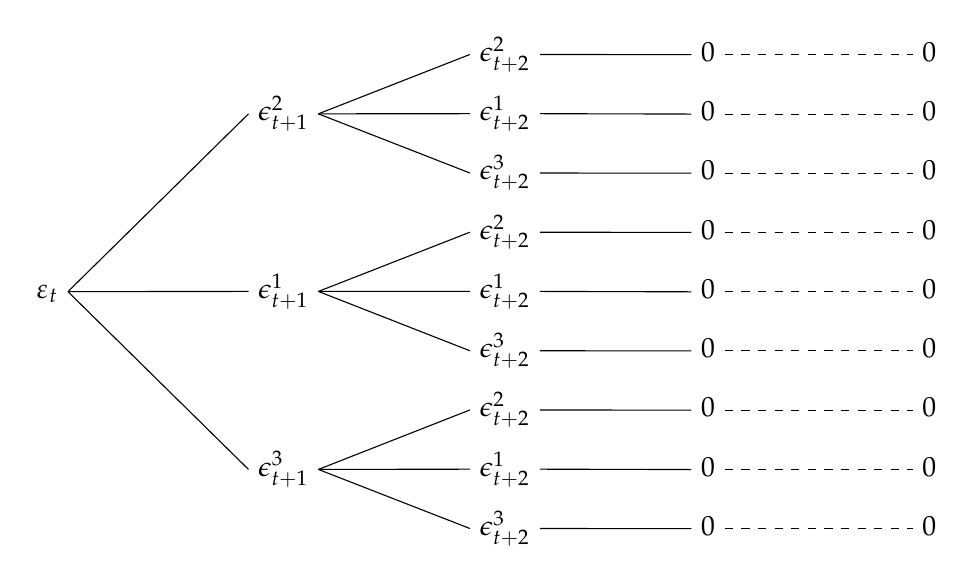
\begin{tikzpicture}
         \tikzset{grow'=right,level distance=80pt}
         \tikzset{execute at begin node=\strut}
         \tikzset{every tree node/.style={anchor=base west}}
         \Tree [.$\varepsilon_t$ [.$\epsilon^2_{t+1}$
         [.{$\epsilon^2_{t+2}$}  [.0 \edge[dashed]; \node{0};] ]
         [.{$\epsilon^1_{t+2}$}  [.0 \edge[dashed]; \node{0};] ]
         [.{$\epsilon^3_{t+2}$}  [.0 \edge[dashed]; \node{0};] ]]
         [.$\epsilon^1_{t+1}$
         [.{$\epsilon^2_{t+2}$}  [.0 \edge[dashed]; \node{0};] ]
         [.{$\epsilon^1_{t+2}$}  [.0 \edge[dashed]; \node{0};] ]
         [.{$\epsilon^3_{t+2}$}  [.0 \edge[dashed]; \node{0};] ]]
         [.$\epsilon^3_{t+1}$
         [.{$\epsilon^2_{t+2}$}  [.0 \edge[dashed]; \node{0};] ]
         [.{$\epsilon^1_{t+2}$}  [.0 \edge[dashed]; \node{0};] ]
         [.{$\epsilon^3_{t+2}$}  [.0 \edge[dashed]; \node{0};] ]]]
      \end{tikzpicture}}
   \bigskip\bigskip
   \caption{\textbf{Paths of  future innovations as a perfect tree.} Stochastic extended path of order $p=2$ with $m=3$ integration nodes. Perfect ternary tree of length 3, followed by sequences of zeros (the leafs). Conditional expectations are estimated at the root of the tree and at three non-terminal nodes (integration nodes in $t+1$). The leafs, after the terminal nodes of the perfect tree (integration nodes in $t+2$), correspond to the deterministic trajectories leading to the steady state for the endogenous variables.}
   \label{fig:sep:tree}
\end{figure}


\begin{figure}[H]
   \centering
   {\tiny
      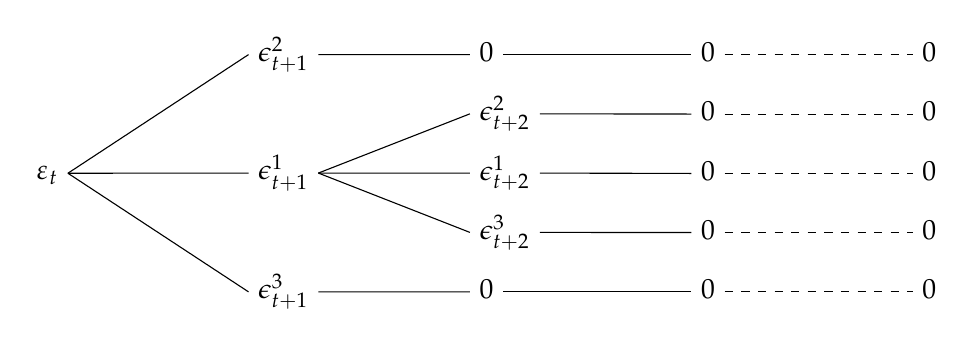
\begin{tikzpicture}
         \tikzset{grow'=right,level distance=80pt}
         \tikzset{execute at begin node=\strut}
         \tikzset{every tree node/.style={anchor=base west}}
         \Tree [.$\varepsilon_t$
         [.$\epsilon^2_{t+1}$ [ .0  [.0 \edge[dashed]; \node{0};]]]
         [.$\epsilon^1_{t+1}$
         [.{$\epsilon^2_{t+2}$}  [.0 \edge[dashed]; \node{0};] ]
         [.{$\epsilon^1_{t+2}$}  [.0 \edge[dashed]; \node{0};] ]
         [.{$\epsilon^3_{t+2}$}  [.0 \edge[dashed]; \node{0};] ]]
         [.$\epsilon^3_{t+1}$ [ .0  [.0 \edge[dashed]; \node{0};]]]]
      \end{tikzpicture}}
   \bigskip\bigskip
   \caption{\textbf{Paths of  future innovations as a sparse tree.} Stochastic extended path of order $p=2$ with $m=3$ integration nodes. Sparse tree of length 2, followed by sequences of zeros (the leafs). Conditional expectations are estimated along the trunk (here in periods $t$ and $t+1$). The leafs, after the terminal nodes of the sparse tree ($\epsilon_{t+1}^2$, $\epsilon_{t+1}^3$, $\epsilon_{t+2}^2$, $\epsilon_{t+2}^1$ and $\epsilon_{t+2}^3$)), correspond to the deterministic trajectories leading to the steady state for the endogenous variables.}
   \label{fig:sep:sparse-tree}
\end{figure}


\begin{figure}[H]
   \centering
   \hspace*{-0.8cm}\scalebox{.85}{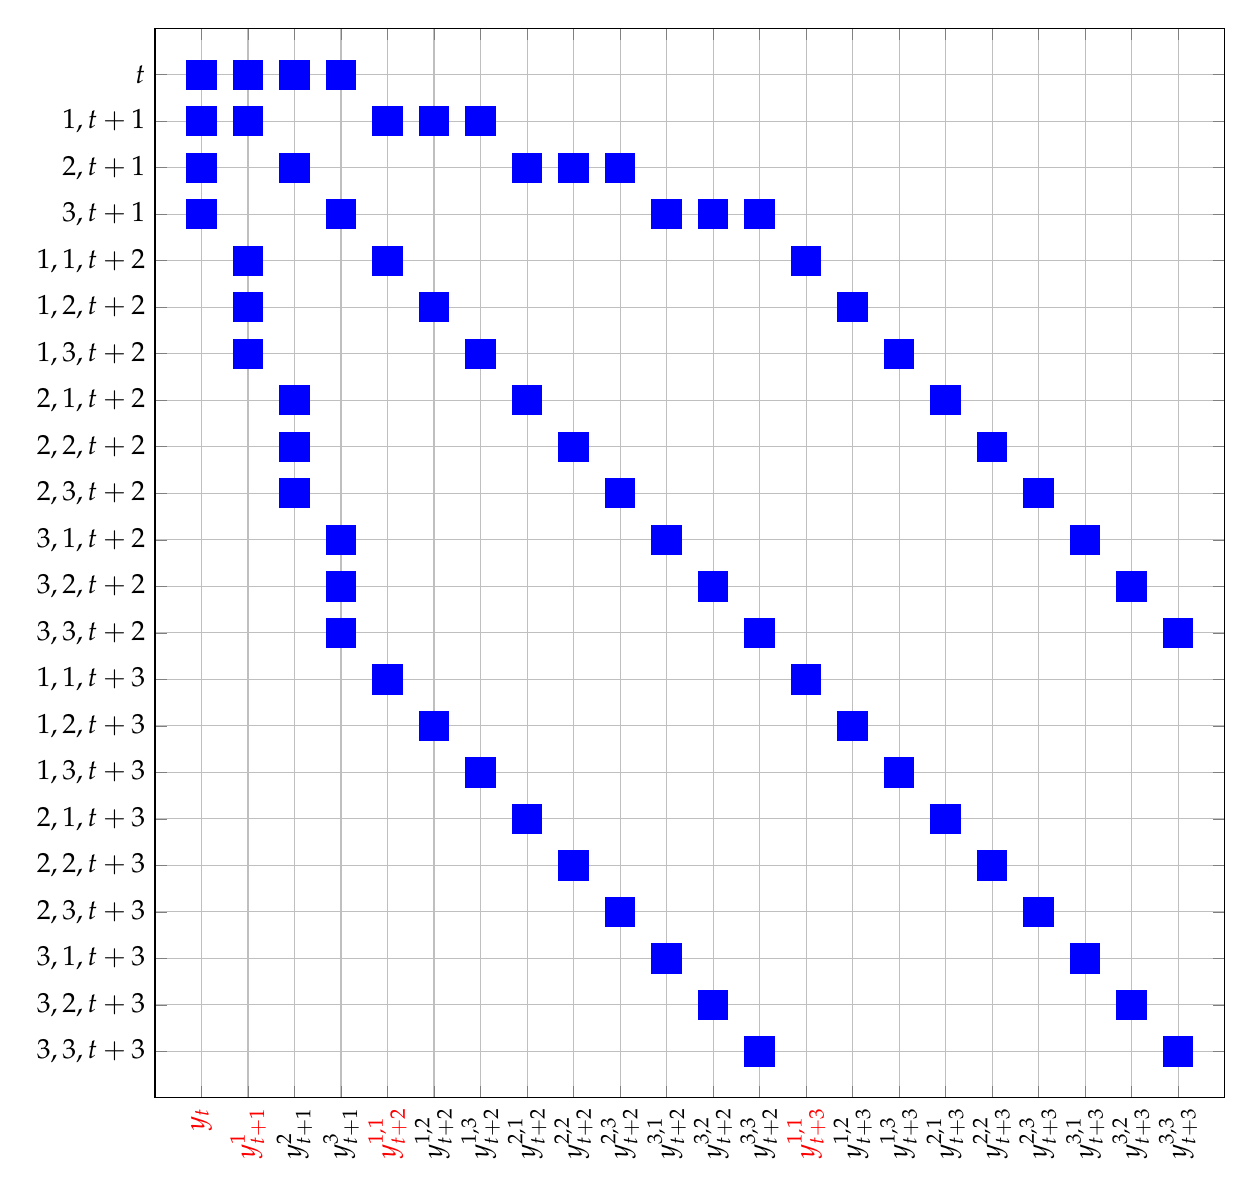
\begin{tikzpicture}

\begin{axis}[%
width=5.348in,
height=5.348in,
at={(1.854in,0.722in)},
scale only axis,
xmin=0,
xmax=23,
xtick={1,2,3,4,5,6,7,8,9,10,11,12,13,14,15,16,17,18,19,20,21,22},
xticklabels={{\color{red}$y_t$},{\color{red}$y_{t+1}^1$},{$y_{t+1}^2$},{$y_{t+1}^3$},{\color{red}$y_{t+2}^{1,1}$},{$y_{t+2}^{1,2}$},{$y_{t+2}^{1,3}$},{$y_{t+2}^{2,1}$},{$y_{t+2}^{2,2}$},{$y_{t+2}^{2,3}$},{$y_{t+2}^{3,1}$},{$y_{t+2}^{3,2}$},{$y_{t+2}^{3,3}$},{\color{red}$y_{t+3}^{1,1}$},{$y_{t+3}^{1,2}$},{$y_{t+3}^{1,3}$},{$y_{t+3}^{2,1}$},{$y_{t+3}^{2,2}$},{$y_{t+3}^{2,3}$},{$y_{t+3}^{3,1}$},{$y_{t+3}^{3,2}$},{$y_{t+3}^{3,3}$}},
xticklabel style={rotate=90},
y dir=reverse,
ymin=0,
ymax=23,
ytick={1,2,3,4,5,6,7,8,9,10,11,12,13,14,15,16,17,18,19,20,21,22},
yticklabels={$t$,{$1,t+1$},{$2,t+1$},{$3,t+1$},{$1,1,t+2$},{$1,2,t+2$},{$1,3,t+2$},{$2,1,t+2$},{$2,2,t+2$},{$2,3,t+2$},{$3,1,t+2$},{$3,2,t+2$},{$3,3,t+2$},{$1,1,t+3$},{$1,2,t+3$},{$1,3,t+3$},{$2,1,t+3$},{$2,2,t+3$},{$2,3,t+3$},{$3,1,t+3$},{$3,2,t+3$},{$3,3,t+3$}},
axis background/.style={fill=white},
xmajorgrids,
ymajorgrids
]
\addplot [color=blue, only marks, mark size=5.3pt, mark=square*, mark options={solid, blue}, forget plot]
  table[row sep=crcr]
   \caption{\textbf{Partial view of the stacked jacobian with a perfect tree.} Stochastic extended path of order $p=2$ with $m=3$. We present only the top-left portion of the Jacobian matrix. Each blue square represents a non zero $n\times n$ block of derivatives. The labels on the horizontal axis illustrate the manner in which the unknown vectors are concatenated to construct the stacked system of equations.}
   \label{fig:jacobian:perfect-tree}
\end{figure}


\begin{figure}[H]
   \centering
   \hspace*{-0.4cm}\scalebox{.85}{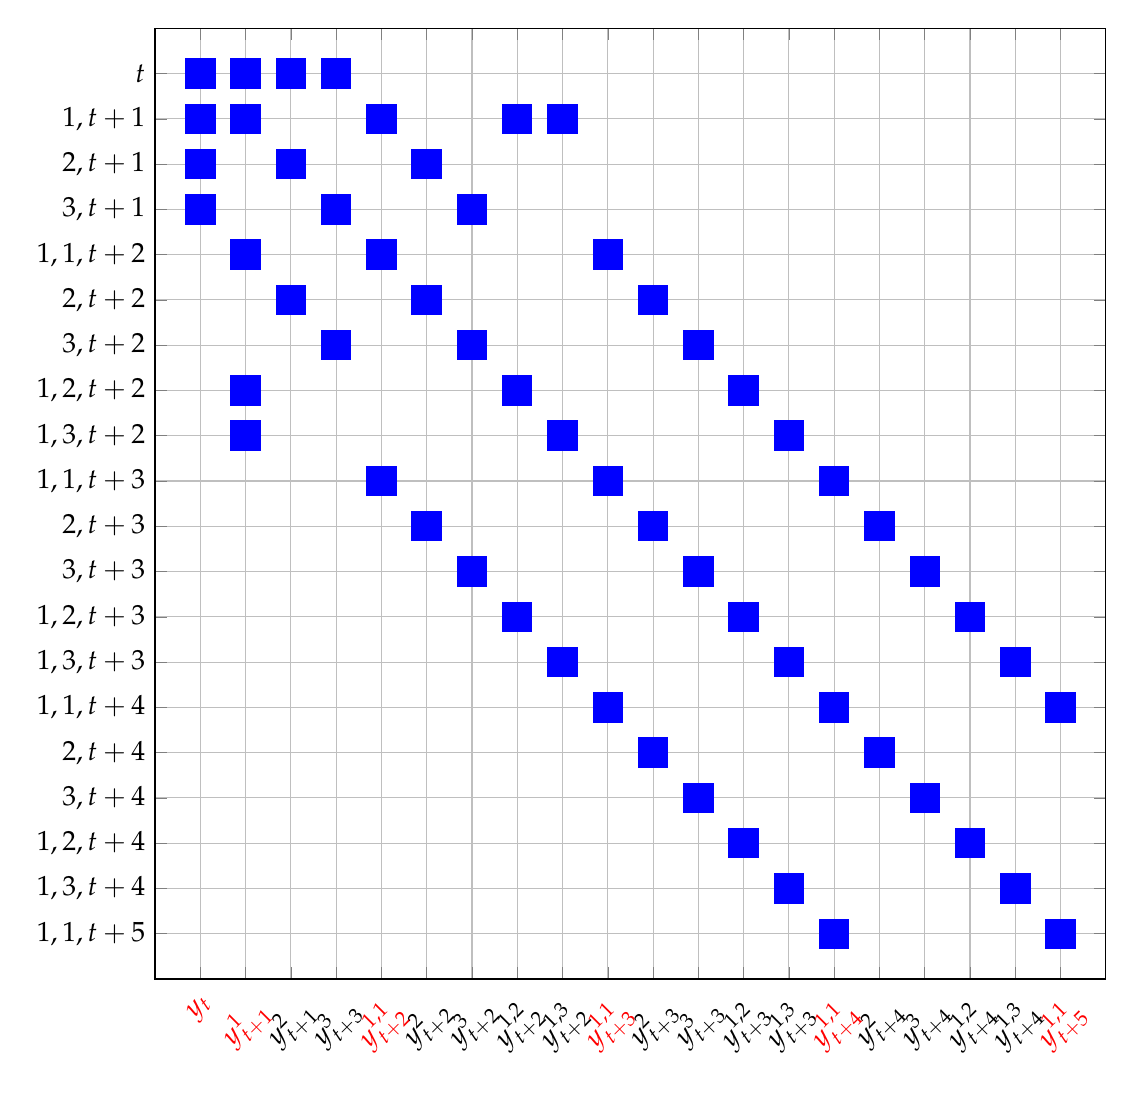
\begin{tikzpicture}

\begin{axis}[%
width=4.754in,
height=4.754in,
at={(1.648in,0.642in)},
scale only axis,
xmin=0,
xmax=21,
xtick={1,2,3,4,5,6,7,8,9,10,11,12,13,14,15,16,17,18,19,20},
xticklabels={{\color{red}$y_{t}$},{\color{red}$y_{t+1}^1$},{$y_{t+1}^2$},{$y_{t+3}^3$},{\color{red}$y_{t+2}^{1,1}$},{$y_{t+2}^2$},{$y_{t+2}^3$},{$y_{t+2}^{1,2}$},{$y_{t+2}^{1,3}$},{\color{red}$y_{t+3}^{1,1}$},{$y_{t+3}^2$},{$y_{t+3}^3$},{$y_{t+3}^{1,2}$},{$y_{t+3}^{1,3}$},{\color{red}$y_{t+4}^{1,1}$},{$y_{t+4}^2$},{$y_{t+4}^3$},{$y_{t+4}^{1,2}$},{$y_{t+4}^{1,3}$},{\color{red}$y_{t+5}^{1,1}$}},
xticklabel style={rotate=45},
y dir=reverse,
ymin=0,
ymax=21,
ytick={1,2,3,4,5,6,7,8,9,10,11,12,13,14,15,16,17,18,19,20},
yticklabels={{$t$},{$1,t+1$},{$2,t+1$},{$3,t+1$},{$1,1,t+2$},{$2,t+2$},{$3,t+2$},{$1,2,t+2$},{$1,3,t+2$},{$1,1,t+3$},{$2,t+3$},{$3,t+3$},{$1,2,t+3$},{$1,3,t+3$},{$1,1,t+4$},{$2,t+4$},{$3,t+4$},{$1,2,t+4$},{$1,3,t+4$},{$1,1,t+5$}},
axis background/.style={fill=white},
xmajorgrids,
ymajorgrids
]
\addplot [color=blue, only marks, mark size=5.3pt, mark=square*, mark options={solid, blue}, forget plot]
  table[row sep=crcr]
   \caption{\textbf{Partial view of the stacked jacobian with a sparse tree.} Stochastic extended path of order $p=2$ with $m=3$. We present only the top-left portion of the Jacobian matrix. Each blue square represents a non zero $n\times n$ block of derivatives. The labels on the horizontal axis illustrate the manner in which the unknown vectors are concatenated to construct the stacked system of equations.}
   \label{fig:jacobian:sparse-tree}
\end{figure}



\newpage

\setcounter{equation}{0}
\renewcommand{\theequation}{\thesection.\arabic{equation}}


\section{Equations of the RBC model}\label{appendix:rbc}
\setcounter{equation}{0}

\begin{equation}
   \label{annex:rbc:efficiency}
   \begin{cases}
      A_t & = A^{\star}e^{a_t}         \\
      a_t & = \rho_a a_{t-1} + u_{a,t}
   \end{cases}
\end{equation}
\begin{equation}
   \label{annex:rbc:euler}
   \begin{split}
       & \left[c_t^{\theta}(1-l_t)^{1-\theta}\right]^{-\tau}\theta c_t^{\theta-1}(1-l_t)^{1-\theta}-\mu_t                                                                              \\ &-
      \beta \mathbb E_t \Biggl[\left[c_{t+1}^{\theta}(1-l_{t+1})^{1-\theta}\right]^{-\tau}\theta c_{t+1}^{\theta-1}(1-l_{t+1})^{1-\theta}                                              \\
       & \times \Biggl\{\alpha \left[\alpha+(1-\alpha)\left(\frac{k_{t+1}}{l_{t+1}}\right)^{-\psi}\right]^{\frac{1-\psi}{\psi}}A_{t+1}+1-\delta\Biggr\}-\mu_{t+1}(1-\delta)\Biggr] = 0
   \end{split}
\end{equation}
\begin{equation}
   \label{annex:rbc:labour}
   \frac{1-\theta}{ \theta}\frac{c_t}{1-l_t} - (1-\alpha)A_t\left[\alpha \left(\frac{k_t}{l_t}\right)^{\psi}+1-\alpha\right]^{\frac{1-\psi}{\psi}} = 0
\end{equation}
\begin{equation}
   \label{annex:rbc:capital_law_of_motion}
   c_t + k_{t+1} - A_t\left[\alpha k_t^{\psi} + (1-\alpha) l_t^{\psi}\right]^{\frac{1}{\psi}}- (1-\delta)k_t = 0
\end{equation}
\begin{equation}
   \label{annex:rbc:excl}
   \mu_t \left(k_{t+1}-(1-\delta)k_t\right) = 0\text{ with }\mu_t\geq 0 \, \forall t
\end{equation}
\newline

Equation (\ref{annex:rbc:efficiency}) is the efficiency law of
motion, (\ref{annex:rbc:euler}) is the Euler equation,
(\ref{annex:rbc:labour}) is the first order condition for labour
supply, (\ref{annex:rbc:capital_law_of_motion}) is physical capital
stock law of motion and (\ref{annex:rbc:excl}) the complementary slackness condition
associated with the positivity constraint on investment.\newline

\end{document}

%%% Local Variables:
%%% mode: LaTeX
%%% TeX-master: t
%%% End:
